%!TEX root = ../Report.tex

% This information is used in titlepage, colophon, preface and hyperref setup (pdf metainfo), and other options.
\def\thesistypeabbr{ }
\def\thesistype    { }

\def\thesisauthor  {Nicolè Lorenzo}
\def\thesistitle   {Appunti}
\def\thesissubtitle{Metallurgia II}
\def\thesislocation{\copyright~Università degli Studi di Ferrara,}

\def\papersize    {a4paper} % Final paper size (b5paper/a4paper), recommended paper size is b5paper
\def\showtrims    {false} % Print on larger paper than \papersize and show trim marks (true/false)?

\def\showtodos    {true}  % Show todos (true/false)?
\def\confidential {true} % Confidential report (true/false)?

% Legal references – UK
\newcommand \legal[2]{\S#1 paragraph #2}





\newcommand{\papersizeswitch}[3]{\ifnum\strcmp{\papersize}{#1}=0#2\else#3\fi}
\papersizeswitch{a4paper}{\def\classfontsize{10pt}}{\def\classfontsize{12pt}}

\documentclass[\classfontsize,\papersize,oneside,extrafontsizes]{memoir}

%!TEX root = ../TecMec.tex 
% \RequirePackage[l2tabu,orthodox]{nag} % Old habits die hard

% \newcommand{\papersizeswitch}[3]{\ifnum\strcmp{\papersize}{#1}=0#2\else#3\fi}
% \papersizeswitch{b5paper}{\def\classfontsize{10pt}}{\def\classfontsize{12pt}}

% \documentclass[\classfontsize,\papersize,twoside,showtrims,extrafontsizes]{memoir}
\RequireXeTeX

\showtrimsoff
\papersizeswitch{b5paper}{
    % Stock and paper layout
    \pagebv
    \setlrmarginsandblock{20mm}{20mm}{*}
    \setulmarginsandblock{35mm}{30mm}{*}
    \setheadfoot{8mm}{10mm}
    \setlength{\headsep}{7mm}
    \setlength{\marginparwidth}{18mm}
    \setlength{\marginparsep}{2mm}
}{
    \papersizeswitch{a4paper}{
        \pageaiv
        \setlength{\trimtop}{0pt}
        \setlength{\trimedge}{\stockwidth}
        \addtolength{\trimedge}{-\paperwidth}
        \settypeblocksize{634pt}{448.13pt}{*}
        \setulmargins{4cm}{*}{*}
        \setlrmargins{*}{*}{1}
        \setmarginnotes{17pt}{51pt}{\onelineskip}
        \setheadfoot{\onelineskip}{2\onelineskip}
        \setheaderspaces{*}{2\onelineskip}{*}
    }{
    }
}
\ifnum\strcmp{\showtrims}{true}=0
    % For printing B5 on A4 with trimmarks
    \showtrimson
    \papersizeswitch{b5paper}{\stockaiv}{\stockaiii}
    \setlength{\trimtop}{\stockheight}
    \addtolength{\trimtop}{-\paperheight}
    \setlength{\trimtop}{0.5\trimtop}
    \setlength{\trimedge}{\stockwidth}
    \addtolength{\trimedge}{-\paperwidth}
    \setlength{\trimedge}{0.5\trimedge}
    
    % bigger todos if trim marks
    \setmarginnotes{10pt}{95pt}{\onelineskip}

    \trimLmarks
    
    % put jobname in left top trim mark
    \renewcommand*{\tmarktl}{%
      \begin{picture}(0,0)
        \unitlength 1mm
        \thinlines
        \put(-2,0){\line(-1,0){18}}
        \put(0,2){\line(0,1){18}}
        \put(3,15){\normalfont\ttfamily\fontsize{8bp}{10bp}\selectfont\jobname\ \
          \today\ \ 
          \printtime\ \ 
          Page \thepage}
      \end{picture}}

    % Remove middle trim marks for cleaner layout
    \renewcommand*{\tmarktm}{}
    \renewcommand*{\tmarkml}{}
    \renewcommand*{\tmarkmr}{}
    \renewcommand*{\tmarkbm}{}
\fi

\checkandfixthelayout                 % Check if errors in paper format!
\sideparmargin{outer}                 % Put sidemargins in outer position (why the fuck is this option not default by the class?)

% Large environments
\usepackage{microtype}
\usepackage{mathtools}
\usepackage{listings}                 % Source code printer for LaTeX
\usepackage[tablegrid,owncaptions]{vhistory}

% Links
\usepackage[hyphens]{url}             % Allow hyphens in URL's
\usepackage[unicode=false,psdextra]{hyperref}                 % References package

% Graphics and colors
\usepackage{graphicx}                 % Including graphics and using colours
\usepackage{xcolor}                   % Defined more color names
\usepackage{eso-pic}                  % Watermark and other bag
\usepackage{preamble/dtucolors}
\graphicspath{{graphics/}}
\usepackage{subfig}
\usepackage{pst-solides3d}
\usepackage{tabularx}
\usepackage{tree}
\usepackage{tikz}

% Math
\usepackage{euler}
\usepackage{amsfonts}
\usepackage{amssymb}

% Custom colors
\definecolor{UnifeLight}{HTML}{00819f}
\definecolor{UnifeDark}{HTML}{1c2c4a}

% Language
\usepackage{polyglossia}    % multilingual typesetting and appropriate hyphenation
\setdefaultlanguage{italian}
\setotherlanguage[variant=american]{english}
\usepackage{csquotes}       % language sensitive quotation facilities
\newcommand{\eng}[1]{\foreignlanguage{english}{#1}}

% Bibliography (references)
\usepackage[backend=biber,
            %backref=true,
            abbreviate=false,
            dateabbrev=false,
            alldates=long]{biblatex}

% Floating objets, captions and references
\usepackage{flafter}  % floats is positioned after or where it is defined! 
%\setfloatlocations{figure}{bhtp}   % Set floats for all figures
%\setfloatlocations{table}{bhtp}    % Set floats for all tables
%\setFloatBlockFor{section}         % Typeset floats before each section
\usepackage[noabbrev,nameinlink,capitalise]{cleveref} % Clever references. Options: "fig. !1!" --> "!Figure 1!"
\hangcaption
\captionnamefont{\bfseries}
\subcaptionlabelfont{\bfseries}
\newsubfloat{figure}
\newsubfloat{table}
%\letcountercounter{figure}{table}         % Consecutive table and figure numbering
%\letcountercounter{lstlisting}{table}     % Consecutive table and listings numbering
\captiontitlefinal{.}
% strip things from equation references, making them "(1)" instead of "Equation~1"
% from http://tex.stackexchange.com/questions/122174/how-to-strip-eq-from-cleveref
\crefformat{equation}{(#2#1#3)}
\crefrangeformat{equation}{(#3#1#4) to~(#5#2#6)}
\crefmultiformat{equation}{(#2#1#3)}%
{ and~(#2#1#3)}{, (#2#1#3)}{ and~(#2#1#3)}

% Table of contents (TOC)
\setcounter{tocdepth}{3}              % Depth of table of content
\setcounter{secnumdepth}{2}           % Depth of section numbering
\setcounter{maxsecnumdepth}{3}        % Max depth of section numbering

% Todos
\usepackage{totcount}                 % For total counting of counters
\def\todoshowing{}
\ifnum\strcmp{\showtodos}{false}=0
    \def\todoshowing{disable}
\fi
\usepackage[colorinlistoftodos,\todoshowing]{todonotes} % Todonotes package for nice todos
\newtotcounter{todocounter}           % Creates counter in todo
\let\oldtodo\todo
\newcommand*{\newtodo}[2][]{\stepcounter{todocounter}\oldtodo[#1]{\thesection~(\thetodocounter)~#2}}
\let\todo\newtodo
\let\oldmissingfigure\missingfigure
\newcommand*{\newmissingfigure}[2][]{\stepcounter{todocounter}\oldmissingfigure[#1]{\thesection~(\thetodocounter)~#2}}
\let\missingfigure\newmissingfigure
\makeatletter
\newcommand*{\mylistoftodos}{% Only show list if there are todos
\if@todonotes@disabled
\else
    \ifnum\totvalue{todocounter}>0
        \markboth{\@todonotes@todolistname}{\@todonotes@todolistname}
        \phantomsection\todototoc
        \listoftodos
    \else
    \fi
\fi
}
\makeatother
\newcommand{\lesstodo}[2][]{\todo[color=green!40,#1]{#2}}
\newcommand{\moretodo}[2][]{\todo[color=red!40,#1]{#2}}

% Chapterstyle
\makeatletter
\makechapterstyle{mychapterstyle}{
    \chapterstyle{default}
    \def\format{\normalfont\sffamily}

    \setlength\beforechapskip{0mm}

    \renewcommand*{\chapnamefont}{\format\HUGE}
    \renewcommand*{\chapnumfont}{\format\fontsize{54}{54}\selectfont}
    \renewcommand*{\chaptitlefont}{\format\fontsize{42}{42}\selectfont}

    \renewcommand*{\printchaptername}{\chapnamefont\MakeUppercase{\@chapapp}}
    \patchcommand{\printchaptername}{\begingroup\color{dtugray}}{\endgroup}
    \renewcommand*{\chapternamenum}{\space\space}
    \patchcommand{\printchapternum}{\begingroup\color{UnifeLight}}{\endgroup}
    \renewcommand*{\printchapternonum}{%
        \vphantom{\printchaptername\chapternamenum\chapnumfont 1}
        \afterchapternum
    }

    \setlength\midchapskip{1ex}

    \renewcommand*{\printchaptertitle}[1]{\raggedleft \chaptitlefont ##1}
    \renewcommand*{\afterchaptertitle}{\vskip0.5\onelineskip \hrule \vskip1.3\onelineskip}
}
\makeatother
\chapterstyle{mychapterstyle}

% Header and footer
\def\hffont{\sffamily\small}
\makepagestyle{myruled}
\makeheadrule{myruled}{\textwidth}{\normalrulethickness}
\makeevenhead{myruled}{\hffont\thepage}{}{\hffont\leftmark}
\makeoddhead{myruled}{\hffont\rightmark}{}{\hffont\thepage}
\makeevenfoot{myruled}{}{}{}
\makeoddfoot{myruled}{}{}{}
\makepsmarks{myruled}{
    \nouppercaseheads
    \createmark{chapter}{both}{shownumber}{}{\space}
    \createmark{section}{right}{shownumber}{}{\space}
    \createplainmark{toc}{both}{\contentsname}
    \createplainmark{lof}{both}{\listfigurename}
    \createplainmark{lot}{both}{\listtablename}
    \createplainmark{bib}{both}{\bibname}
    \createplainmark{index}{both}{\indexname}
    \createplainmark{glossary}{both}{\glossaryname}
}
\pagestyle{myruled}
\copypagestyle{cleared}{myruled}      % When \cleardoublepage, use myruled instead of empty
\makeevenhead{cleared}{\hffont\thepage}{}{} % Remove leftmark on cleared pages

\makeevenfoot{plain}{}{}{}            % No page number on plain even pages (chapter begin)
\makeoddfoot{plain}{}{}{}             % No page number on plain odd pages (chapter begin)

% \*section, \*paragraph font styles
\setsecheadstyle              {\huge\sffamily\raggedright}
\setsubsecheadstyle           {\LARGE\sffamily\raggedright}
\setsubsubsecheadstyle        {\Large\sffamily\raggedright}
%\setparaheadstyle             {\normalsize\sffamily\itseries\raggedright}
%\setsubparaheadstyle          {\normalsize\sffamily\raggedright}


% Hypersetup
\hypersetup{
    pdfauthor={\thesisauthor{}},
    pdftitle={\thesistitle{}},
    pdfsubject={\thesissubtitle{}},
    pdfdisplaydoctitle,
    bookmarksnumbered=true,
    bookmarksopen,
    breaklinks,
    linktoc=all,
    plainpages=false,
    unicode=true,
    colorlinks=false,
    citebordercolor=dtured,           % color of links to bibliography
    filebordercolor=dtured,           % color of file links
    linkbordercolor=dtured,           % color of internal links (change box color with linkbordercolor)
    urlbordercolor=s13,               % color of external links
    hidelinks                         % Do not show boxes or colored links.
}

% Hack to make right pdfbookmark link. The normal behavior links just below the chapter title. This hack put the link just above the chapter like any other normal use of \chapter.
% Another solution can be found in http://tex.stackexchange.com/questions/59359/certain-hyperlinks-memoirhyperref-placed-too-low
\makeatletter
\renewcommand{\@memb@bchap}{%
  \ifnobibintoc\else
    \phantomsection
    \addcontentsline{toc}{chapter}{\bibname}%
  \fi
  \chapter*{\bibname}%
  \bibmark
  \prebibhook
}
\let\oldtableofcontents\tableofcontents
\newcommand{\newtableofcontents}{
    \@ifstar{\oldtableofcontents*}{
        \phantomsection\addcontentsline{toc}{chapter}{\contentsname}\oldtableofcontents*}}
\let\tableofcontents\newtableofcontents
\makeatother

% Confidential
\newcommand{\confidentialbox}[1]{
    \put(0,0){\parbox[b][\paperheight]{\paperwidth}{
        \begin{vplace}
            \centering
            \scalebox{1.3}{
                \begin{tikzpicture}
                    \node[very thick,draw=UnifeDark!#1,color=UnifeDark!#1,
                          rounded corners=2pt,inner sep=8pt,rotate=-20]
                          {\sffamily \HUGE \MakeUppercase{Confidential}};
                \end{tikzpicture}
            }
        \end{vplace}
    }}
}

% Prefrontmatter
\newcommand{\prefrontmatter}{
    \pagenumbering{alph}
    \ifnum\strcmp{\confidential}{true}=0
        \AddToShipoutPictureBG{\confidentialbox{10}}   % 10% classified box in background on each page
        \AddToShipoutPictureFG*{\confidentialbox{100}} % 100% classified box in foreground on first page
    \fi
}

% DTU frieze
\newcommand{\frieze}{%
    \AddToShipoutPicture*{
        \put(0,0){
            \parbox[b][\paperheight]{\paperwidth}{%
                %\includegraphics[trim=130mm 0 0 0,width=0.9\textwidth]{tex_DTU_frise}
                %\vspace*{2.5cm}
                \includegraphics[width=0.5\textwidth]{graphics/UnivAQ_logoA.eps}
                \vspace*{5cm}
            }
        }
    }
}
% This is a double sided book. If there is a last empty page lets use it for some fun e.g. the frieze.
% NB: For a fully functional hack the \clearpage used in \include does some odd thinks with the sequence numbering. Thefore use \input instead of \include at the end of the book. If bibliography is used at last everything should be ok.
\makeatletter
% Adjust so gatherings is allowed for single sheets too! (hacking functions in memoir.dtx)
\patchcmd{\leavespergathering}{\ifnum\@memcnta<\tw@}{\ifnum\@memcnta<\@ne}{
    %\leavespergathering{1}
    % Insert the frieze
    %\patchcmd{\@memensuresigpages}{\repeat}{\repeat\frieze}{}{}
}{}
\makeatother

% Custom comands
\usepackage{multicol}
%!TEX root = ../Report.tex 

% Text fonts (http://www.macfreek.nl/memory/Fonts_in_LaTeX)
% Install fonts from /usr/local/texlive/<version>/texmf-dist/fonts/opentype/public
\usepackage{fontspec}

% Sans-serif font
\setsansfont[
    Ligatures=TeX,
    Extension=.otf,
    UprightFont=*-regular,
    BoldFont=*-bold,
    ItalicFont=*-italic,
    BoldItalicFont=*-bolditalic,
    %SlantedFont=,
    %BoldSlantedFont=,
    %SmallCapsFont=
    Scale=0.8      % Adjustmens when using math in sections
]{texgyreadventor}
%\setsansfont[Ligatures=TeX]{Neo Sans Intel}    % Neo Sans Intel – Like DTU font but more symbols
%\setsansfont[
%    Ligatures=TeX,
%    Scale=0.8
%]{NeoSans}           % NeoSans – DTU font (missing `+' symbols and other)
%\setsansfont[Ligatures=TeX]{CMU Sans Serif}    % Computer Modern Unicode font
%\setsansfont[Ligatures=TeX]{Latin Modern Sans} % Latin Modern Sans serif font

% Use this for more convienent sans serif font in math mode.
%\setmathsf{Latin Modern Sans}


%!TEX root = ../Report.tex 

% Content specific packages.

\usepackage{blindtext}
\usepackage{algorithm}
\usepackage{algpseudocode}
\usepackage{pgfplots}                 % Plot tools
\usetikzlibrary{
    arrows,
    matrix,
    positioning,
    shapes,
    topaths,
}
\pgfplotsset{compat=1.7}

% Listings
\lstset{
    basicstyle=\footnotesize\ttfamily,% the size of the fonts that are used for the code
    breakatwhitespace=false,          % sets if automatic breaks should only happen at whitespace
    breaklines=true,                  % sets automatic line breaking
    captionpos=b,                     % sets the caption-position to bottom
    commentstyle=\color{s14a},        % comment style
    deletekeywords={},                % if you want to delete keywords from the given language
    escapeinside={\%*}{*)},           % if you want to add LaTeX within your code
    frame=single,                     % adds a frame around the code
    keywordstyle=\bfseries\ttfamily\color{s09}, % keyword style
    language=Python,                  % the language of the code
    morekeywords={*,...},             % if you want to add more keywords to the set
    numbers=left,                     % where to put the line-numbers; possible values are (none, left, right)
    numbersep=5pt,                    % how far the line-numbers are from the code
    numberstyle=\sffamily\tiny\color{dtugray}, % the style that is used for the line-numbers
    rulecolor=\color{dtugray},        % if not set, the frame-color may be changed on line-breaks within not-black text (e.g. comments (green here))
    showspaces=false,                 % show spaces everywhere adding particular underscores; it overrides 'showstringspaces'
    showstringspaces=false,           % underline spaces within strings only
    showtabs=false,                   % show tabs within strings adding particular underscores
    stepnumber=1,                     % the step between two line-numbers. If it's 1, each line will be numbered
    stringstyle=\color{s07},          % string literal style
    tabsize=2,                        % sets default tab size to 2 spaces
    title=\lstname,                   % show the file name of files included with \lstinputlisting; also try caption instead of title
}

\usepackage{pdflscape}
\usepackage{acronym}
%\usepackage{natbib}
\usepackage{amsmath}
\usepackage{enumitem}

\addbibresource{bibliography/bibliography.bib}

\begin{document}

\prefrontmatter
%!TEX root = ../MatMetII.tex
\thispagestyle{empty}             % No page numbers
\calccentering{\unitlength}
\begin{figure}[h!]
    \hfill
\includegraphics[height=1.8cm]{graphics/DE}
    %\hspace{0.5cm}
    %
\includegraphics[height=1.8cm]{graphics/DE}
\end{figure}
\begin{adjustwidth*}{\unitlength}{-\unitlength}
    \begin{adjustwidth}{-0.5cm}{-0.5cm}
        \sffamily
        \begin{flushright}
            %\thesistypeabbr{}\\*[0cm]
        \end{flushright}
        \vspace*{\fill}
        \noindent
        %\includegraphics[width=0.25\textwidth]{LINX_QIM}\\*[0.5cm]
        \HUGE \thesistitle{}\\*[0.2cm]
        \Huge \thesissubtitle{}\\*[1.2cm]
        \parbox[b]{\linewidth}{%
            \LARGE 
            %\thesisauthor{}\\*[1.2cm]
            \normalsize
            \thesislocation{} \the\year
        }
    \end{adjustwidth}
\end{adjustwidth*}
\normalfont
\normalsize

\cleartoevenpage
%!TEX root = ../Report.tex 
\thispagestyle{empty} % No page numbers
%\frieze
\vspace*{\fill}
\sffamily

\Large{
\noindent
\textbf{DE}\\
\textbf{Department of Engeneering Ferrara}\\
}

\small
\noindent
\textbf{Via Saragat 1, 44122 Ferrara}\\
\textbf{https://de.unife.it/it}\\
\\
Università degli Studi di Ferrara\\
%Polo Tecnico-Scientifico\\
Via Ludovico Ariosto, 35 - 44121 Ferrara\\
https://www.unife.it/it\\
\normalsize
\normalfont
\vspace*{2.5cm}

\clearforchapter
%!TEX root = ../MatMetII.tex
% Start of the revision history table
\def\vhhistoryname{Revisioni}%
\def\vhversionname{Revisione}%
\def\vhdatename{Data}%
\def\vhauthorname{Autori}%
\def\vhchangename{Descrizione}%

\begin{versionhistory}
  \vhEntry{1.0}{29.01.2021}{XX YY}{document created}
  \vhEntry{1.1}{06.03.2023}{LN}{Prima compilazione con modifiche}
  \vhEntry{1.2}{15.03.2023}{LN}{Completamento Capitolo 1}
\end{versionhistory}

\vspace{3cm}

\noindent\large\textbf{Università degli Studi di Ferrara}\\

\noindent\normalsize [XX] Dr. Name Surname - name.surname@xxx.com\\
\noindent\normalsize [YY] Dr. Name Surname - name.surname@xxx.com\\
\noindent\normalsize [LN] Lorenzo Nicolè - \href{mailto:lorenzo.nicole@edu.unife.it}{lorenzo.nicole@edu.unife.it}
\clearforchapter

\frontmatter
%\chapter{Abstract}
\noindent Il presente \ac{TR} ...
%\chapter{Prefazione}
...
%\chapter{Acknowledgements}
\noindent Il presente \ac{TR} ...
\clearforchapter
\tableofcontents
\clearforchapter
\listoffigures
\clearforchapter
\listoftables
\clearforchapter
\mylistoftodos

\mainmatter
\part{Introduzione}
\chapter{Classificazione e Designazione degli acciai}\label{chp:ClassAcc}
\section{La normazione}
Per cominciare, è utile osservare come gli enti di normazione descrivono gli acciai.
tra l'altro sono tra i prodotti più normati presenti sul mercato industriale.
Dapprima:
\begin{description}
\item[UNI] sigla che indica una normativa realizzata dall'Ente nazionale di Unificazione.
Ente che norma tutte le attività produttive sul mercato italiano. Inoltre è facente parte del \acs{CEN}. Difatti applica sul suolo italiano tutte le normative date dallo stesso \acs{CEN}.
Non è ammessa la presenza di normative che siano in contrasto con quelle europee.
\item[EN] contraddistingue le norma sviluppate dal \ac{CEN}.
Le normative EN devono essere percepite da tutti gli stati membri dello spazio economico europeo.
Ciò per garantire il libero scambio di prodotti al interno del mercato.
Il EN è composto dai principali enti nazionali di normazione degli stati membri nello spazio economico europeo.
\item[ISO] rappresenta tutte le normative sviluppate dal \ac{ISO}. Possono essere un riferimento applicabile per tutto il mondo. Una nazione può decidere se applicare le norma \acs{ISO} indipendentemente da quanto fatto dal \acs{CEN}.
\end{description} 

Secondo le normative della \acs{CEN} le normative hanno lo scopo di:
\begin{quote}
Stabilire le condizioni tecniche per lo scambio di prodotti e di servizi assicurando il continuo adeguamento allo sviluppo delle tecnologie e dei bisogni del mercato
\end{quote}
con lo scopo di eliminare le barriere commerciali, almeno tra gli stati europei.

Una prima classificazione dei tipi di acciai perché esistono tante classi di materiale.
Dunque si può pensare ad una divisione in base:
\begin{multicols}{2}
\begin{itemize}
\item composizione chimica;
\item processo di fabbricazione;
\item caratteristiche meccanico-fisiche e di impiego;
\columnbreak
\item costituenti strutturali;
\item ecc\dots
\end{itemize}
\end{multicols}

Non a caso sono stati citati i precedenti aspetti, in fatti le normative vanno a coprire gli aspetti stessi, come mostrato nella tabella \ref{tab:NormGen}

\begin{table}
\centering
\caption{Norme di carattere geneale}\label{tab:NormGen}
\begin{tabularx}{\textwidth}{>{\bfseries}lX}
\toprule
UNI EN 10020:2001 & Descrizione e classificazione dei tipi di acciaio\\
UNI EN 10027-1:2016 & Sistemi di designazione degli acciai, \texttt{Designazione alfanumerica}\\
UNI EN 10027-2:2015 & Sistemi di designazione degli acciai, \texttt{Designazione numerica}\\
UNI EN 10025-(1-6):2005 & Prodotti laminati a caldo di acciai per impieghi strutturali\\
UNI EN 10079:2007 & Descrizione dei prodotti di acciaio (forma, dimensioni, aspetto, stato superficiale)\\
\bottomrule
\end{tabularx}
\end{table}

Secondo la norma \texttt{UNI EN 10020:2001}:
\begin{quote}
L'acciaio è un materiale il cui \emph{tenore in massa di Ferro (Fe) è maggiore di quello di ciascuno degli altri elementi} ed il cui \emph{tenore di Carbonio (C) è generalmente minore del $2\%$} e che contiene altri elementi. Un numero limitato di acciai al Cromo (Cr) può avere tenore di carbonio maggiore del $2\%$, ma tale valore del $2\%$ è il tenore limite corrente che separa l'acciaio dalla ghisa.
\end{quote}
Sempre la stessa norma definisce la classificazione principale degli acciai \ref{fig:UNIEN10020:2001}.

\begin{figure}
\usetikzlibrary{trees}
\begin{tikzpicture}[
sibling distance = 10em,
every node/.style={rectangle, rounded corners, draw, align=center,}
]
\node{Acciai}
	child{ node[top color = UnifeLight] {Non legati}
		child{ node[bottom color = UnifeDark!80, white] {di qualità}}
		child{ node[bottom color = UnifeDark!80, white] {speciale}}}
	child{node[top color = UnifeLight] {Inossidabili}}
	child{node[top color = UnifeLight] {Legati}
		child{node[bottom color = UnifeDark!80, white] {di qialità}}
		child{node[bottom color = UnifeDark!80, white] {speciali}}};
\end{tikzpicture}
\caption{Suddivisione acciai in base alla normativa UNI EN 10020:2001}
\label{fig:UNIEN10020:2001}
\end{figure}
Dove:
\begin{itemize}
\item \textcolor{UnifeLight}{$\blacksquare$} è la suddivisione per composizione chimica;
\item \textcolor{UnifeDark!80}{$\blacksquare$} è la suddivisione in base alle caratteristiche meccanico-fisiche della suddivisione chimica.
\end{itemize}
L'appartenenza ad una classe si basa sulla composizione chimica di colata indicata sulla norma di prodotto, prendendo in considerazione il valore minimo.
Vediamo ora come vengono suddivise le categorie in base alla norma.
\begin{description}
\item[Acciai non legati] sono gli acciai per cui \emph{Nessuno dei valori limite, rigorosamente fissati dalla norma (tabella \ref{tab:Prosp1}), è raggiunto dai rispettivi tenori degli elementi in lega} (escluso il C).
\item[Acciai inossidabili] sono acciai contenenti \emph{almeno il $10.5\%$ di Cr e al massimo l'$1.2\%$ di C}.
\item[Acciai legati] sono acciai per i quali \emph{almeno uno dei valori limite è raggiunto dai dai rispettivi tenori degli elementi in lega} (tabella \ref{tab:Prosp1}) a patto che non siano già appartenenti agli inossidabili.
\end{description}

\begin{table}
\centering
\caption{Prospetto I, norma UNI EN 10020:2001}\label{tab:Prosp1}
\begin{tabularx}{0.5\textwidth}{lXl}
\toprule
\textbf{Elemento} &\textbf{Tenore in $\%$ in massa}\\
\midrule
Al & Alluminio & 0.30\\
B & Boro & 0.0008\\
Bi & Bismuto & 0.10\\
Co & Cobalto & 0.30\\
Cr & Cromo & 0.30\\
Cu & Rame & 0.40\\
La & Lantanidi (singolarmente) & 0.10\\
Mn & Manganese & 1.65\\
Mo & Molibdeno & 0.08\\
Nb & Niobio & 0.06\\
Ni & Nichel & 0.30\\
Pb & Piombo & 0.40\\
Se & Selenio & 0.10\\
Si & Silicio & 0.60\\
Te & Tellurio & 0.10\\
Ti & Titanio & 0.05\\
V & Vanadio & 0.10\\
W & Tungsteno & 0.30\\
Zr & Zircronio & 0.05\\
- & Altri & 0.10\\
\bottomrule
\end{tabularx}
\end{table}

\subsection{Acciai non legati}
\begin{multicols}{2}[]
\subsubsection{Di Qualità}
Sono acciai per i quali, in genere, sussistono prescrizioni riguardanti caratteristiche specifiche, per esempio: tenacità, grossezza e/o formabilità.
Non sono destinati a trattamenti termici (al più a ricottura e normalizzazione).
\columnbreak
\subsubsection{Speciali}
Sono acciai che presentano, rispetto agli acciai non legati di qualità, una maggiore purezza in particolare nei confronti delle inclusioni non metalliche.
In genere presentano risposta regolare ai \ac{TT}, e nella maggior parte dei casi sono destinati a:
\begin{enumerate}
\item trattamento di bonifica,
\item trattamento di tempra superficiale.
\end{enumerate}
Fanno parte di tale classe gli acciai non legati che rispondono a una o più delle seguenti prescrizioni tutte quelle definizioni che rientrano in \ref{sec:ANLS}. \todo{Aggiungere i riferimenti all'apendice}
\end{multicols}

\subsection{Acciai inossidabili}
Sono suddivise in base a due criteri:
\begin{enumerate}
\item tenore di Nichel:
\begin{itemize}
\item Ni $<2.5\%$
\item Ni $>2.5\%$
\end{itemize}
\item caratteristiche paricolari:
\begin{itemize}
\item resistenza alla corrosione;
\item resistenza all'ossidazione a caldo;
\item resistenza allo scorrimento.
\end{itemize}
\end{enumerate}
\newpage
\subsection{Acciai legati}
\begin{multicols}{2}[]
\subsubsection{di Qualità}
Sono acciai il cui utilizzo è simile agli acciai non legati di qualità, ma che contengono elementi in lega per rispondere ad alcune prescrizioni di impiego.
Non sono, di regola, destinati a trattamento termico di bonifica o ad un tratamento di tempra superficiale.
Ne fanno parte gli acciai definiti in \ref{sec:ALDQ}.
\columnbreak
\subsubsection{Speciali}
Sono acciai , diversi dagli inossidabili, che non rientrano tra le categorie definite per gli acciai legati di qualità caratterizzati da:
\begin{itemize}
\item regolazione precisa della composizione chimica;
\item particolari condizioni di elaborazione e controllo del processo produttivo.
\end{itemize}
Ne fanno parte gli acciai descritti in \ref{sec:ALS}.
\end{multicols}

\section{La norma UNI EN 10027:2016}
La normativa ha lo scopo di designare univocamente gli acciai disponibili in commercio in base a due modalità: designazione alfanumerica (parte 1) e designazione numerica (parte 2).
Inoltre specifica le modalità di nomenclatura degli acciai: specificando le modalità di ottenimento dei nomi per entrambe le parti%
\footnote{Come nominare un acciaio non viene deciso dall'azienda che lo produce. Lo stesso ente ha il compito di nominare gli acciai.}.
Inizieremo dalla prima parte ovvero quella alfanumerica.
\subsection{UNI EN 10027:2016 parte 1}
Nella prima parte della normativa vengono designati gli acciai in base al loro impiego e alle loro caratteristiche meccanico-fisiche.
Alla figura \ref{tab:Simb} è rappresentata la modalità di nomenclatura alfanumerica.

\begin{table}
\centering
\caption{Indicazioni simboli}\label{tab:Simb}
\begin{tabularx}{\textwidth}{p{0.2\textwidth}XXp{0.1\textwidth}}
\toprule
\textbf{W} & \textbf{X} & \textbf{YYY} & \textbf{ZZ}\\
Simbolo iniziale & Simbolo Impiego & Caratteristiche meccanico-fisiche & Altre indicazioni\\
\midrule
\begin{description}
\item[G]: Acciaio per getti 
\item[PM]: metallurgia delle polveri
\end{description}
&
\begin{description}
\item[S] Impieghi strutturali,
\item[P] Impieghi sotto pressione,
\item[E] Costruzioni meccaniche,
\item[D] Formatura a freddo,
\item[B] Cemento armato,
\item[Y] Cemento armato precompresso,
\item[R] Acciaio per rotaie,
\item[M] Acciai magnetici,
\item[\dots]\dots
\end{description}
&
\begin{description}
\item[$R_{s,min}$] in $\left[ \unit{\MPa}\right]$
\item[$R_{m,min}$] in $\left[\unit{\MPa}\right]$
\item[$HBW_{min}$] (adimensionale)
\end{description}
&
Simboli addizionali divisi in due gruppi
\\
\bottomrule
\end{tabularx}
\end{table}

Come si vede dalla tabella \ref{tab:Simb} i vari simboli occupano una posizione ben determinata e specifica.
C'è da considerare una particolarità tra il simbolo d'impiego e il valore della caratteristica meccanico-fisica specificata per tale categoria.
\begin{description}
\item[In generale] viene specificato il valore di snervamento minimo garantito: $R_{s,min}\left[\unit{MPa}\right]$.
\item[Per Y] Viene specificata la tensione minima di rottura: $R_{m,min}\left[\unit{MPa}\right]$
\item[Per M] Viene indicata una proprietà magnetica (descritta dalla normativa).
\item[Per R] La durezza.
\end{description}
Per quanto riguarda le altre indicazioni, anche in questo caso dipende dal impiego del materiale.
Viene riportato un esempio in tabella \ref{tab:ValRes}.

\begin{table}
\centering
\caption{Valori di resilienza}\label{tab:ValRes}
\begin{tabularx}{\textwidth}{XXXX}
\toprule
\multicolumn{4}{c}{Resilienza}\\
\textbf{J} & \textbf{K} & \textbf{L} & \textbf{Temperatura}\\
min $27\unit{\J}$ & min $40\unit{\J}$ & min $60\unit{\J}$ & $\left[\unit{\celsius}\right]$\\
\midrule
JR & KR & LR & 20\\
J0 & K0 & L0 & 0\\
J2 & K2 & L2 & -20\\
\bottomrule
\end{tabularx}
\end{table}

Se consideriamo come esempio l'acciaio $S355J2$, questo sarà:
\todo{\\Costruire un ambiente adatto per evidenziare gli esempi}
\begin{description}
\item[$S$] un acciaio per impieghi strutturali,
\item[$355$] avrà valore minimo di snervamento pari a $R_{s,min} = 355\unit{\MPa}$,
\item[$J2$] valore di resistenza minima a $27\unit{\J}$ ad una temperatura di $-20\unit{\celsius}$.%
\footnote{Il valore di resilienza dipende dalla temperatura di esercizio del materiale in quanto la bassa temperatura tende a cristallizzare il metallo rendendolo più fragile.}
\end{description}
Tra le altre cose il metallo appena visto è uno di quei metalli facente parte della normativa UNI EN 10025-2 ovvero per gli acciai \textit{prodotti laminati a caldo per impieghi strutturali}. Giusto per darne un accenno la normativa è divisa in sei parti:
\begin{enumerate}
\item Condizioni tecniche generali di fornitura
\item Condizioni tecniche di fornitura di acciai non legati per impieghi strutturali
\item Condizioni tecniche di fornitura di acciai per impieghi strutturali saldabili a grano fine allo stato normalizzato/normalizzato laminato
\item Condizioni tecniche di fornitura di acciai per impieghi strutturali saldabili a grano fine ottenuti mediante laminazione termomeccanica
\item Condizioni tecniche di fornitura di acciai per impieghi strutturali con resistenza migliorata alla corrosione atmosferica
\item Condizioni tecniche di fornitura per prodotti piano di acciai per impieghi strutturali ad alto limite di snervamento allo stato bonificato
\end{enumerate}
\todo[inline]{Designazione con normativa precedente.} %Introduzione agli acciai
\part{Acciai da costruzione}
\chapter{Capitolo}
\label{chp:2}
 %Acciai da costruzione
\chapter{Acciai Speciali da Costruzione}\label{chp:SpecCostruzione}
Sono acciai che vengono caratterizzati tramite la composizione chimica
infatti questi acciai sono spesso trattati con successivi
trattamenti termici prima di essere messi in opera.

In generale vengono classificati tra:
\begin{itemize}
\item Acciai da costruzione propriamente detti;
\item Acciai inossidabili;
\item Acciai da utensili.
\end{itemize}

\section{Acciai speciali da costruzione propriamente detti}
Sono acciai calmati che spesso vengono legati con diversi elementi che donano
particolari capacità tipo: temprabilità, tenacità, buon compromesso tra
tenacità e resistenza meccanica, resistenza all'usura e altre\dots
Come accennato prima spesso vengono applicati dopo aver subito un trattamento 
termico (tempra + rinvenimento).
In genere son impiegati per applicazioni che devono resistere a elevate 
sollecitazioni dinamiche e statiche.

Questi vengono ulteriormente suddivisi secondo l'impiego.
\begin{itemize}
\item Acciai da bonifica,
\item Acciai da cementazione,
\item Acciai da nitrurazione,
\item Acciai per molle,
\item Acciai per cuscinetti,
\item Acciai "automatici",
\item Altri (acciai da bulloneria)\dots
\end{itemize}

In generale sulle schede tecniche degli acciai si trovano degli intervalli 
con dei valori nominali di composizione chimica. Alcuni riferimenti si posso 
trovare nelle varie normative tipo la \texttt{UNI EN 10027} ed eventuali 
normative prodotto aggiuntive.
Inoltre, viene accompagnato con la lista dei trattamenti termici che il 
materiale ha subito ed eventuali caratteristiche meccaniche che si sono 
raggiunte.

Le motivazioni dietro a questa non precisa specificità della composizione
del materiale è dovuta al fatto che ci sono diverse variabili che incorrono 
per il raggiungimento degli obbiettivi meccanici.
Dunque è difficile effettivamente stimare la composizione chimica.

\subsection{Acciai da Bonifica}
Gli acciai da bonifica sono acciai che subiscono un trattamento termico
tipo quello in figura \ref{fig:AccBonifica}.

\begin{figure}
\centering
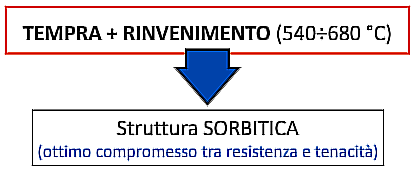
\includegraphics[width = 0.5\textwidth]{AccBonifica}
\caption{Trattamento termico per gli acciai da bonifica}
\label{fig:AccBonifica}
\end{figure}

Gli acciai da bonifica sono adatti, in relazione alla loro composizione 
chimica, per sopportare sforzi, urti e vibrazioni, infatti di solito
si realizzano:
\begin{itemize}
\item Alberi motore,
\item assi,
\item pignoni,
\item bielle,
\item rotismi,
\item ecc\dots
\end{itemize}
Infatti sono parti della macchina che devono possedere delle buone
resistenze a carichi elevati ed alta tenacità. %Acciai Speciali da costruzione
\part{Acciai Inossidabili}
%%%%%%%%%%%%%%%%%%%%%%%%%%%%%%%%%%%%%%%%%%%%%%%%%%%%%%%%%%%%%%%%%%
% Capitoli già visti a lezione								    %
%%%%%%%%%%%%%%%%%%%%%%%%%%%%%%%%%%%%%%%%%%%%%%%%%%%%%%%%%%%%%%%%%%
\newpage
\section{Acciai inossidabili austenitici}
\subsection{Tattamenti termici applicabili}
Durante un'eventuale saldatura, il processo di raffreddamento non è 
controllato per cui non si è sicuri se il processo di stabilizzazione sia 
ancora valido. Perciò è meglio optare per degli acciai low carbon.
Per gli acciai austenitici la sensibilizzazione avviene ad una certa distanza 
dal cordone di saldatura. Per quelli feritici invece si avvicina al cordone
per via delle caratteristiche dell'acciaio.

\subsubsection{Trattamento di distensione}
Si riscalda l'acciaio ad una temperatura inferiore alla temperatura di inizio
sensibilizzazione. Tenendo il processo per circa $30min \div 2h$.
Successivo raffreddamento in aria calma. 
Si fa per eliminare le tensioni interne generate per qualsiasi motivo.
Ciò riduce il pericolo della \emph{tensocorrosione}.
Il processo si esegue solo in caso in cui si presume che ci sia tale moti vo 
di corrosione.

Gli acciai inox austenitici non hanno particolari caratteristiche meccaniche 
Risultano però molto deformabili e hanno una buona capacità di incrudimento.
È possibile che si vada a generare l'effetto \ac{TRIP} (visto in precedenza).
Per via del fatto che essendo deformato a freddo, c'è la tendenza che 
l'austenite venga trasformata in martensite (Sotto la temperatura $M_d$ 
ovvero quella temperatura che permette la trasformazione di austenite in
martensite a fronte di una deformazione).

\missingfigure{Inserire i grafici delle proprietà meccaniche degli 
austenitici}

Gli acciai austenitici hanno una buona resistenza al Creep ovvero
uno sforzo ad alta temperatura a carico costante.

Riassumendo:\\
Gli acciai inossidabili austenitici hanno un buon comportamento a bassa 
temperatura in quanto non presentano la transizione duttile-
fragile. Ad alta temperatura bisogna stare attenti alle temperature  
critiche di sesibilizzazione.
Possono resistere bene alla corrosione in ambienti aggressivi.
Sono molto utilizzati in quei campi dove la sicurezza è di 
fondamentale importanza.

I super-austenitici vengono chiamati così perché hanno valori di $PREN>40$.


\section{Acciai inossidabili ferritici}
Sono ancora acciai monofasici. Secondo l'\ac{AISI} sono 
designati come 4XX. Non è completamente indicativa della struttura in
quanto ci sono sia i ferritici che i martensitici con la stessa nomenclatura.

La tipica lega dei ferritici prevede leghe: Fe-C-Cr.
Dunque si scelgono questi acciai quando si vuole optare per una scelta più 
economica.
Hanno struttura ferritica a tutte le temperature. Fanno eccezione gli acciai
detti \emph{semiferritici} che se scaldati e portati in austenitizzazione 
e raffreddati velocemente formano della martensite.
In genere non sono adatti ai trattamenti termici. E sottoporli a tali 
trattamenti compromette la resistenza a corrosione.
Sono suscettibili al rinforzo per incrudimento, comunque meno di quanto fanno 
gli austenitici.
Un acciaio ferritico di riferimento è l'\texttt{\ac{AISI} 430}.
\missingfigure{Aggiungere Metallografia AISI 442}

\todo[inline]{Vedi la tabella della comparazione delle proprietà}

Possibile formazione della fase $\sigma$ che contiene molto cromo 
andando ad infragilire la struttura e sensibilizza alla corrosione 
intergranulare.

\subsection{Trattamenti termici}
Non si vanno a migliorare le caratteristiche meccaniche come per gli 
asutenitici. Piuttosto vengono tamponate delle situazioni in cui gli 
acciai potrebbero essere più sensibili.

\subsubsection{Ricottura di ricristallizzazione}
Si effettua per ricristallizzare un materiale che precedentemente ha subito 
una deformazione plastica.
Non si deve mai superare la temperatura critica dei $850\unit{\celsius}$ per 
cui il grano ferritico tenderebbe a ingrossare troppo.
Siccome stiamo effettuando una ricristallizzazione non è detto che si possa 
effettuare una successiva deformazione (soprattutto se il pezzo è già 
stato formato).
Si preferisce abbondare col raffreddamento, di solito fatto in acqua.
Perché si può incorrere in fenomeni di infragilimento.
\begin{description}
\item[Infragilimento a $457\unit{\celsius}$] Si ha una decomposizione della 
fase $\alpha$. Da lì inizia a formarsi, per via dell'alta percentuale di 
cromo, da cui si forma sia fase $\alpha$ che $\alpha'$.
Dove la prima è molto ricca di Fe, l'altra più ricca di Cr.
Se ne moficano le caratteristiche meccaniche e aumenta la TTDF%
\todo{acronimo}.
È un problema reversibile, si può scaldare nuovamente il materiale per 
poi raffreddarlo più velocemente.
\item[Infragilimento per fase $\sigma$] È reversibile, in maniera simile 
a quanto visto prima. Bisogna stare attenti alla temperatura di 
riscaldamento che deve essere $\approx 800\unit{\celsius}$. 
\end{description}

Ciò pone questi acciai in situazioni di sensibilizzazione
che può verificarsi a $T > 950\unit{\celsius}$. Perciò bisogna porre 
particolare attenzione alle saldature.

La motivazione è ancora in fase di studio. Perciò non è completamente chiara.
\missingfigure{Aggiungere i grafici della sensibilizzazione}
Si potizza che: a causa della non omogeneità della matrice del materiale, si 
vadano a formare delle isole austenitiche interne al grano ferritico.
Allora possono formarsi dei carburi di ferro che precipitano, risultando più 
sensibili alla corrosione.
Non esiste un processo di stabilizzazione del materiale, perché il processo
di sensibilizzazione non è strettamente legato alla precipitazione di 
carburi di cromo. Perciò non è così efficace.

\subsubsection{Acciai ferritici ELI}
Si tratta di leghe Fe-Cr-Mo a bassisimi tenori di C e N.
Presentano alta resistenza alla tensocorrosione.

\section{Acciai inossidabili Martensitici}
Si applicano per quelle applicazioni in cui si vuole una buona resistenza
alla corrosione (ben maggiore dei CORTEN) ma non si vuole rinunciare
alle caratteristiche meccaniche.
\todo{Aggiungere i tenori di carbonio}
Sono scuscettibili ai trattamenti termici di indurimento in quanto presentano 
i punti critici $A_1$ e $A_3$. 
Dopo la tempra presentano una struttura martensitica o martensitica con 
carburi. Per cui si raggiungono durezze molto elevate $\approx 45\unit{HRC}
\div 65\unit{HRC}$.

Non sono facili da saldare in quanto i tenori di carbonio sono parecchio 
elevati.

Una designazione tipica di riferimento è l'\texttt{AISI 410}.

\subsection{Trattamenti termici}
\todo[inline]{vedi slides per magiore completezza}

Hanno elevata temprabilità e vengono in genere temprati in olio e in aria, 
detti anche autotempranti (la scelta dipende dagli spessori).

\section{Acciai inossidabili PH}

Acciai non più monofasici, andando ad interrogare gli acciai duplex.
\emph{Precipitation Hardening}. 
Sono stati sviluppati per richieste dell'industria aeronautica e bellica.
Hanno elevate caratteristiche meccaniche al contempo elevate caratteristiche
alla corrosione.
Tali caratteristiche si sono ottenute grazie al processo di indurimento per
precipitazione.
Spesso vengono nominati tramite il nome commerciale piuttosto della
designazione normativa.
Secondo l'AISI \todo{Acronimo} sono la serie 6XX. Come riferimento al
\texttt{AISI 630}.

Si nota, dalla nomenclatura europea, che i tenori di carbonio è molto
molto basso $0.01\%$ per alcune formulazioni.
Questa caratteristica non è troppo distante dagli acciai austenitici.
Ciò impone che le caratteristiche meccaniche vengano demandate ai (molti)
elementi in lega. Si demanda alla precipitazione di altre soluzioni.
Ad esempio spesso si hanno precipitazioni tipo: $Ni_3X$ dove $X$ è un
altro elemento in lega.
 %Acciai Inox
\part{Acciai per utensili}
\chapter{Acciai da utensile}\label{chp:Utensili}
Sono utilizzati per la lavorazione o la generazioen della forma dei materiali metallici e non.
Le lavorazioni a cui devono adempire possono essere:
\begin{itemize}
\item Asportazione di materiale
\item Deformazione plastica a caldo
\item Deformazione plastica a freddo
\end{itemize}

Le principali proprietà spesso contrastanti fra le quali trovare un compromesso sono;
\begin{itemize}
\item durezza,
\item resistenza all'usura e all'abrasione,
\item mancanza di fragilità
\end{itemize}

Spesso per gli acciai da utensili si stimano in base alla loro durata: tanto più riesce a mantenere le sue caratteristica, meglio è.
In molti casi non viene specificata un parametro definito. Si cerca di farli durare il più possibile donandogli determinate caratteristiche gli permettono di sopportare una maggiore usura a fronte della lavorazione per cui sono studiati.

\begin{quote}
Quanti tipi di acciai per utensili esistono?
\end{quote}

Ne esistono di molteplici formazioni, leghe ecc\dots in base alle necessità della lavorazione.
Alcuni sono più adatti per la lavorazione a freddo, alcuni mantengono una durezza residua ad alta temperatura (temperatura di flash) nel tempo, alta resistenza all'abrasione, ecc\dots
Caso per caso si hanno esigenze diverse per cui si sono sviluppati acciai corrispondenti.
Tipo:
\begin{description}
\item[Acciai a basso C] per esempio il C40U, è un acciaio a basso tenore di carbonio ottimizzato per la realizzazione da utensili.
\item[Acciai debolmente legati] Anche in questo caso ottimizzati in base alla lavorazione che devono eseguire
\item[Acciai fortemente legati] Si parla di un tenore di elementi leganti che arriva fino al 30\%.
\end{description}

Di particolare importanza diventano i trattamenti termici, in base a questi uno stesso acciaio può ottenere proprietà diverse.
Per esempio, gli acciai rapidi sono acciai che possono lavorare altri acciai, ottimizzati per lavorare ad alta velocità.

Di particolare importanza per questi acciai è sicuramente la purezza e la sequenza delle fasi di produzione dell'acciaio.

Il rendimento dell'utensile dipende particolarmente da:
\begin{enumerate}
\item Appropriata progettazione dell'utensile,
\item Accuratezza nella produzione dell'utensile,
\item Selezione accurata dell'acciaio più adatto allo scopo,
\item Corretta esecuzione del trattamento termico più appropriato.
\end{enumerate}

\todo[inline]{Citazione delle proprietà più richieste}

La durezza dell'utensile deve essere maggiore del materiale da lavorare. Non è sempre vero, o meglio va adattato alla lavorazione. In genere si sceglie una differenza di durezza tra i due acciai di circa un centinaio di Viskers.
La resistenza all'usura è un discorso complesso, indicativamente dipende dall'affinità tra i due materiali. Se i due metalli lo sono, l'utensile tenderà a durare meno.
La resistenza a fatica viene suddivisa tra:
\begin{description}
\item[Resistenza a fatica meccanica] in cui per ovviare a tale problema si agisce più sulla conformazione dell'utensile piuttosto del materiale.
\item[Resistenza a fatica termica] Dovuto ai cicli di produzione, ad esempio in presso-fusione dell'alluminio, in cui ne risente la finitura superficiale. Vale anche nel caso di utensili per asportazione. Prevalentemente è più problematica questa fatica perché gli utensili vengono più compressi che non trazionati.
\end{description}
Anche per questi acciai valgono le classiche relazioni tra durezza-duttilità e tenacità.
la temprabilità non è da sottovalutare sempre in termini di garantire delel caratteristiche meccaniche non indifferenti per questi acciai.
Attenzione all'aggiunta "compulsiva" di elementi di lega per aumentare la temprabilità. Di solito si abbassa la conduttività termica: si rischia di andare a formare delle cricche a caldo sia in salita di temperatura che in spegnimento. Per cui è necessario controllare il mezzo di spegnimento.
Ingrossando il grano si elimina una delle poche strategie per tenere duttile l'acciaio. Gli elementi in lega tendono ad irrigidire molto l'acciaio perdendo di tenacità. Per cui ingrossare troppo i grani per surriscaldamento non è cosa buona.

Negli acciai da utensili gli elementi in lega possono essere divisi in 2 gruppi:
\begin{description}
\item[Elementi che formano carburi] Cr, Mo, W, V, Ti
\item[Elementi che non formano carburi] Si, Ni, Mn, Co
\end{description}
\todo{\\Riorganizzare La descrizione precedente per abbellirla}
I vari elementi non vengono mai usati da soli ma agiscono in maniera sinergica.
Molti degli elementi possono avere circa lo stesso effetto: la scelta tra i vari può essere fatto su prove sperimentali o on base al costo della lega.

I carburi che si formano sia sostituendo il Fe nella cementite che tramite carburi particolari tipo: $MC$, $M_2C$, $M_3C$, $M_6C$, $M_7C_3$\dots
Tutti questi carburi sono più duri della cementite:
\begin{itemize}
\item aumentano la durezza e la resistenza all'usura
\item rallentano l'addolcimento durante il rinvenimento, fondamentale per gli acciai per utensili per lavorazioni a caldo 
\item I carburi hanno una minore velocità di coalescenza inferiore rispetto alla cementite.
\end{itemize}
Per avere la massima precipitazione fine e dispersa di carburi è necessaria la massima dissoluzione del carbonio nell'austenite.

\missingtable{Tabella tipologie di carburi ottenibili}
\missingfigure{Diagramma resistenza carburi}
Ai carburi è richiesto di avere un periodo di coalescenza il più lungo possibile.

Gli acciai da utensili possono presentare il \texttt{Picco di durezza secondaria} ovvero un picco di durezza, alle volte superiore, per via delle alte capacità di resistenza al rinvenimento. Ciò è dovuto grazie alla precipitazione di alcuni carburi che avendo una velocità di diffusione modesta, che avviene solamente per temperature alte, allora si ha la precipitazione dei carburi proprio a quelle temperature in cui rinviene: per cui aumenta la durezza generale dell'acciaio. 

Per gli elementi che non formano carburi
In particolare il Co non forma mai carburi solidi. In più, rallenta la velocità di rinvenimento rallentando anche tutte quelle trasformazioni che avvengono durante il rinvenimento. Riduce però la temprabilità.
\todo{\\Aggiungere anche gli altri elementi}

\section{Trattamenti termici}
Vediamo il tipico trattamento termico per gli acciai da utensili potrebbe essere:
\missingfigure{Grafico trattamento termico acciai utensili}
Ipotizzando di utilizzare un acciaio particolarmente legato.
Si parte dalla colata di una lingotto o lingottino%
\footnote{Si utilizzano dei piccoli stampi di colata perché alto legaggio corrisponde ad una bassa condittività termica. Quindi per evitare che il materiale si fratturi durante il raffreddamento allora si preferisce realizzare dei lingotti molto piccoli}
e lo si raffredda al interno dello stampo. 
In fase di prima solidificazione si potrebbero ottenere strutture dendritica che presenta una maglia inter-dendritica caratterizzata dalla presenza di carburi. I carburi in prima solidificazione sono i residui della fase di prima solidificazione. Saranno, dunque, generati direttamente dal liquido: detti anche \textit{primari}. Per sciogliere i carburi bisogna riportare il materiale ad una temperatura prossima a quella di fusione del materiale. Però non si vuole arrivare a quel punto perché se si manda l'acciaio vicino alla fusione si rischia di \emph{bruciare l'acciaio}.
A quello stato conviene rifondere tutto.
La maglia non la si vuole. Si ha una zona del materiale che è particolarmente dura riducendo la tenacità.
Allora si cerca di rompere la struttura dendritica e la maglia di carburi.
Il processo di deformazione plastica a caldo viene detto \textbf{impastamento}. Inoltre si vuole evitare un incolonnamento dei carburi: altrimenti si avrebbe un materiale decisamente anisotropo.
Segue una fase di ricottura, a temperatura più bassa della temperatura di lavorazione a caldo. Segue un raffreddamento controllato lente.
Si va a fare la formatura dell'utensile.
In fine di esegue una sorta di distensione per rilassare il materiale.
Dopo può seguire il trattamento termico per la specifica caratteristica ricercata.

Il trattamento termico successivo prevede tre fasi:
\missingfigure{Trattamento termico di indurimento}
\begin{enumerate}
\item Austenitizzazione,
\item Tempra,
\item Rinvenimento doppio o addirittura triplo.
\end{enumerate}
Il trattamento di indurimento viene eseguito post distensione perché data la bassa conduttività termica, se si scalda il materiale mentre presenta delle tensioni residue per via delle lavorazioni a freddo si rischia di creare delle fratture del materiale.

\todo[inline]{Aggiungi lezione del 21/04/2023} %Acciai per utensili
\part{Ghise}
\chapter{Ghise}\label{chp:Ghise}
Le ghise sono dei prodotti ferrosi, contenenti un alto tenore di carbonio.
Cioò conferisce proprietà completamente diverse dagli acciai, permettendo di raggiungere lo stato liquido a temperature più basse $\approx 1200\unit{\celsius}$. Sono particolarmente adatte alla lavorazione per colata.
Iteressano tutti i settori ingegneristici. 
Si considera una ghisa con tenore di carbonio $2.5\% \leq \%C \leq 4.5\%$.
è anche notevolmente superiore al massimo di solubilità dell'austenite alla temperatura eutettica.
Data l'elevata fragilità, non sono in genere lavorabili per deformazione plastica né a caldo né a freddo.
Possiedono delle proprietà che possono essere variate in larga misura in relazione alla lega, in funzione del controllo della produzione ed eventuale trattamento termico.

\missingfigure{Altoforno}
Dall'altoforno si ottengono sempre delle ghise in prima colata a partire da:
\begin{itemize}
\item Minerale di ferro
\item \eng{Coke} metallurgico
\item Vari fondenti
\end{itemize}
Si hanno diverse trasformazioni nel tino del forno si ottengono;
\begin{description}
\item[Ghisa] che verrà successivamente:
	\begin{itemize}
	\item Produzione di acciaio, in ciclo integrato
	\item Realizzazione dei getti in ghisa
	\end{itemize}
\item[Scorie] che vengono utilizzate per la realizzazione di altri materiali.
\end{description}
Dopo il processo in altoforno dove si ottiene la prima ghisa, si passano ad altri processi che permettono di ottenere dei prodotti più elaborati.
Quasi la totalità di getti viene ottenuta tramite prodotta tramite ghise di seconda fusione.

\missingfigure{Grafico fonderie di seconda fusione}

\section{Il materiale}
\missingfigure{Inserire grafico Fe-C}

Il carbonio è presente siamo come cementite sia come grafite, il che porta ad avere differenze microstrutturali e di proprietà.

\begin{description}
\item[Cementite]\todo{\\Aggiungere}
\item[Grafite]
\end{description}
%Da quotare
Come si possono classificare le ghise?

\begin{enumerate}
\item In base allo stato in cui è presente il carbonio
	\begin{itemize}
	\item Ghise bianche: solo $Fe_3C$
	\item Ghise grafitiche: presenza anche di carbonio grafitico 
	\end{itemize}
\item Se grafitiche in base alla forma della grafite: lamellare, nodulare, sferoidale, vermiculare.
\item In base alle proprietà: es. \texttt{EN GJS 500-7} dove viene indicato il tipo di ghisa, il carico di rottura ed eventualmente l'allungamento percentuale a rottura.
\end{enumerate}

\begin{description}
\item[Ghisa bianca] Il carbonio si presenta in forma $Fe_3C$; durante la solidificazione e il raffreddamento segue il diagramma di stato metastabile Fe-C.
\item[Ghisa grigia lamellare] Sarà presente del carbonio libero sotto forma di lamelle (grafite lamellare): la maggior parte del carbonio (tutto in senso ingegneristico) precipita durante la solidificazione sotto forma di lamelle di grafite.
\item[Ghisa grigia sferoidale] Il carbonio è largamente non combinato, si presenta sotto forma di sferoidi regolari di grafiti. Gli sferoidi csi ottengono per opportuno trattamento del fuso grazie ad aggiunte di elementi come $Ce$\todo{\\Completare}
\item[Ghise malleabili] sono quasi in disuso, sostituite dalle sferoidali. Il carbonio si presenta quasi tutto sotto forma di particelle di geometria tondeggiante ed irregolare. Questa morfologia è ottenuta mediante \ac{TT} delle ghise bianche con lo scopo di conferire duttilità.
\item[Ghise conchigliate o temprate] sono delle ghise grigie, per il fatto che non vengono colate in stampo in terra ma in uno stampo metallico, la velocità di raffreddamento è molto più elevata per via del più alto scambio termico con lo stampo. Si favorisce il raffreddamento secondo il grafico metastabile. La pelle del colato sarà prevalenemente a fase cementite. Il cuore del materiale si hanno gradienti di raffreddamento più tranquilli, infatti si ottiene della comune ghisa grigia.
\item[Ghise legate] Si utilizzano dei leganti per modificare la struttura durante il raffreddamento. Si va a stabilizzare una determinata fase a temperatura ambiente.
\end{description}

\missingfigure{Micrografie ghisa grigia, sferoidale}

\section{Fattori di influenza}
I fattori che influenzano il modo di presentarsi del carbonio nelle ghise:
\begin{itemize}
\item Composizione chimica;
\item Eventuale trattamento della ghisa fusa, detto inoculazione;
\item Velocità di raffreddamento;
\item Eventuale \ac{TT}.
\end{itemize}

Elementi come il $Si$ e basse velocità di raffreddamento sono fattori grafitizzanti.

\missingfigure{Diagramma di stato Fe-C-Si}

Aggiungere, per esempio il 2\% di $Si$ permette di traslare tutto il grafico Fe-C verso sinistra. Di conseguenza sposta la percentuale di carbonio che da la composizione eutettoidica e alza l'eutettoide.
Questo permette anche di aumentare il divario tra struttura eutettica stabile e metastabile. Per cui durante il raffreddamento il materiale ha la tendenza a formare più grafite.\todo{\\Aggiungere punti importanti del grafico Fe-C-Si}
A questo proposito si è sviluppato un parametro di carbonio equivalente che tiene in considerazione di questo effetto del silicio che viene usato per considerare una ghisa ipoeutettica, ipereutettica ecc\dots

Ne corso di un generico raffreddamento si potrebbe raggiungere l'eutettico metastabile solo con un sottoraffreddamento molto più rapido di quello stabile. Quindi si ha un effetto grafitizzante.
Al contrario il $Cr$ ha un effetto \textbf{antigrafitizzante}.
\todo{\\Aggiungere gli elementi grafitizzanti e antigrafitizzanti}

Se si mantiene costante uguale a 1 il rapporto tra silicio e cromo si ha un intervallo di eutettico stabile e metastabile costante decrescente.
Il fosforo è vero che è un elemento grafitizzante ma permette di abbassare di molto la temperatura di solidificazione: aumentando la colabilità della lega.

\subsection{Il carbonio equivalente}
Senza silicio la composizione dell'eutettico è pari al 4.3\% di C. 
All'aumentare del tenore di silicio diminuisce il tenore di carbonio dell'eutettico
\begin{equation}
CE = \%C + \frac{\%Si}{3}
\label{eqn:CarbEquivGhise}
\end{equation}
Per esempio per ogni 1\% di Si, la composizione eutettica viene ridotta di 0.3\% di C come si può vedere dalla \eqref{eqn:CarbEquivGhise}.
Quindi quando $CE = 4.3\%$ allora la lega è eutettica. Ghise con uguale CE possono essere ottenute con diversi rapporti di $C$ e $Si$.
Ne caso di composizione ad alto tenore di fosforo, essendo anche lui un elemento grafitico, si aggiunge nella considerazione del CE come nell'equazione \eqref{eqn:CarbEquivGhiseFosforo}.
\begin{equation}
CE = \%C + \frac{\%Si}{3} + \frac{\%P}{3}
\label{eqn:CarbEquivGhiseFosforo}
\end{equation}
\missingfigure{Grafico posizionamento delle ghise in funzione del C-Si}

\subsection{Solidificazione e raffreddamento}
Considerando una ghisa ipoeutettoidica, $CE \lesssim 4.0\%$valutiamo il raffreddamento presentato al grafico 
\missingfigure{Grafico raffreddamento}

\todo[inline]{aggiungi slide considerazioni sul raffreddamento}

\subsection{Inoculazione}
Ha il compito di controllare il numero di celle eutettiche e le modalità di solidificazione (stabile-metastabile) privilegiando la fase grafitica.
Gli inoculati vengono utilizzati in presenza di elevati sottoraffreddamenti tali da provocare la formazione di cementite o alterare la distribuzione della grafite.
Gli inoculanti sono delle ferroleghe $Fe-Si + Ca + Ba + Al + Sr + Zr$
\todo{\\Porre come definizione o esempio per evidenziare.}
Questi formano dei composti che servono da nuclei eterogenei per la formazione della grafite.
Vengono versati in siviera di colata, in percentuali dello $0.3\div1\%$ (in più si ritarda l'inoculazione prima della colata, maggiore è l'effetto).
Bisogna considerare un tempo di "evanescenza" altrimenti le ferroleghe si disciolgono nella composizione del liquido di tutta la ghisa vanificando il tentativo di inoculare.
\missingfigure{Nucleazione grafite + Strutture grafite}
la grafite risulta molto suscettibile allo sfaldamento per via delle modalità di interconnessione sei vari strati di grafene: i vari strati sono legati tramite forze di Van Der Waals. Per cui i legami sono deboli ed è molto facile romperli.

Volendo osservare il cambio di fase specifico per ogni struttura che la ghisa a raggiungere, partiamo dall'austenite.

\section{Solidificazione e raffreddamento}
Si ha una prima formazine di dendriti di austenite primaria per via del sottoraffreddamento rispetto a $T_L$.

Ci sono molte teorie sulla nucleazione e sull'accrescimento dell'eutettico $\gamma - C$.
Una delle teorie più accreditate si basa sul concetto delle \textit{celle eutettiche}:
\begin{itemize}
\item Nuclei di grafite si formano nel liquido e nel liquido impoverito 
\todo{\\Completa}
\end{itemize}
\missingfigure{Modalità accrescimento grafite}
\todo[inline]{Recuperare il materiale}
Siccome il carbonio dovrebbe attraversare una fase $\gamma$ per passare dal liquido al nucleo di grafite.\todo{\\Fino a qua}

La grafite vermiculare si ottiene tramite tentativo di inoculazione sferoidale riuscito male o non completamente. Per cui il risultato è un vermicello invece della sfera attesa. Non è sempre una cosa negativa: alcune ghise vermiculari vengono tutt'ora usate per componentistica di pompe oleodinamiche a pressione. Viene anche chiamata ghisa compatta.

Dopo il completamento della solidificazione dell'eutettico, ci si ritrova con un materiale contenente austenite e grafite.
Raffreddando ulteriormente tra la temperatura eutettica e eutettoidica si ha espulsione del carbonio dall'austenite che andrà accumulato nelle vicinanze della grafite già solidificata. Si forma allora della ferrite nelle prossimità dei nuclei grafitici nel caso in cui la lega sia fortemente grafitizzante. Se invece la ghisa è in condizioni antigrafitizanti tende a nucleare cementite.
\missingfigure{Inizio nuclazione ferrite + micrografie}

Gli elementi in lega hanno una notevole influenza anche nel promuovere le diverse strutture al raffreddamento dopo solidificazione:
\begin{description}
\item[Promotori ferrite] Si, Al,
\item[Promotori perlite] Sn, Mn, Cr, Ni, Sb, Cu,
\item[Affinatori perlite] Ni, Mo, V,
\item[Effetti sinergici tra i vari elementi in lega]
\end{description}
Gli elementi in lega non vanno aggiunti singolarmente ma vanno soppesati tra loro per ottenere, giostrandosi tra la forcella degli elementi in lega permessi dalla normativa, specifiche caratteristiche meccaniche richieste dal cliente.

Tale spaziatura è influenzata dalle condizioni di raffreddamento del getto.
La distanza $\lambda$ tra le lamelle di perlite ha effetto sulla durezza.
\missingfigure{Grafico distanza lamelle - durezza}

\section{Classificazione delle ghise}
\subsection{Classificazione della grafite}
La grafite viene classificata di:
\begin{description}
\item[Forma] lamelle, sferoidi, compatta;
\item[Distribuzione] uniforme, interdendritica, a rosette, \dots
\item[Dimensioni] da $1\unit{\mm}$ a $0.015\unit{\mm}$
\end{description}
La classificazione viene normata da \texttt{ASTM A247 (1967)}, \texttt{UNI 3775 (1973)}, \texttt{UNI EN ISO 945-1:2018}.
La classificazione può essere fatta sia ad occhio con piccoli ingrandimenti, sia attraverso degli opportuni misuratori digitali che restituiscono i vari parametri secondo normativa.

La classificazione è in numeri romani che identificano le varie casistiche. Vanno da I a VI in base alla forma.
\missingfigure{Possibili forme grafite}
Per la distribuzione, nel solo caso I, si utilizzano delle lettere da A a E come mostrato in figura.
\missingfigure{Possibili distribuzioni grafite caso I}
Per quanto riguarda dimensione si usa una cifra da $1 \div 8$. Si valutano 
le dimensioni della lamella o dello sferoide.
Per gli sferoidi si misurano i diametri per quanto possibile, mentre per le lamelle si misura una specie di corda.
\todo{\\Aggiungi eventuali esempi di codifica della grafite}

\subsection{Classificazione della matrice}
Le possibili matrici possono essere:
\begin{description}
\item[Martensitica]\todo{\\come si ottiene}
\item[Austenite]\todo{\\come si ottiene}
\end{description}

\subsection{Classificazione complessiva}
la normativa di riferimento è la \texttt{UNI EN 1560:2011}
\todo[inline]{Da porre come definizione come fatto in precedenza}
\missingtable{Classificazione generale ghisa}
Qui di seguito portati alcuni degli esempi \todo{\\Aggiungi gli esempi}
Esiste anche una designazione numerica in forma 5.XXXX
\missingtable{Aggiungere nomenclatura numerica}

\section{Ghise bianche}
Hanno impiego non particolarmente interessante dal punto di vista ingegneristico per via del fatto che tutto il carbonio è recluso nella cementite, per cui queste ghise vengono usate soprattutto per applicazioni lavoranti in compressione.
Eventualmente vengono prodotte per ottenere le ghise malleabili. Anche se pure le ultime sono ormai soppiantate.
\missingfigure{Metallografie ghise bianche}

\section{Ghise grigie}
Sono tra i materiali ferrosi più utilizzati, soprattutto tra le ghise.
Il loro nome è dato dalla colorazione grigiastra assunta dalla loro superficie di frattura.
La loro struttura \todo{\\completa}

Sono identificate tramite EN + GJL + 100 dove le cifre rappresentano il valore di tensione a rottura del materiale. Non viene specificato l'eventuale allungamento elastico per via del fatto che raramente hanno un comportamento elastico.
\missingtable{Ghise grigie normate}
\missingfigure{metallografie ghise grigie}
Nella vecchia normativa si sfruttava una notazione più tecnica tipo \texttt{G25} o \texttt{G00}\footnote{Non era garantita alcuna proprietà meccanica}.
La sterlite è una struttura eutettoidica ternaria particolarmente carica di fosforo. ha una struttura simile alla ledeburite per via delle macchie a leopardo presenti nella struttura.

Proprietà meccaniche. Risulta pure difficile definire un modulo elastico per via delle bassissime deformazioni. Tant'è che il modulo elastico viene calcolato matematicamente e non attraverso snervamento.

\todo[inline]{Aggiungere trattamenti termici}

\section{Ghise Sferoidali}
\todo[inline]{Aggiungere le sferoidali}
Cerio non è un vero e proprio neutralizzante per neutralizzare elementi di lega che tenderebbero a formare grafite in forma lamellare invece di sferoidale.
Durante la solidificazione la grafite precipita sotto forma di sferoidi o noduli più o meno regolari.
Date le caratteristiche può sostituire acciai da costruzione con tutti i vantaggi portati dalle ghise.

\subsection{Produzione della ghisa}
Per la produzione delle ghise si effettua un processo simile alla deossidazione vista per la calmatura degli acciai, in questo caso si parla di desolforazione perché è un elemento favorente la grafite lamellare piuttosto della sferoidale.

\subsection{La sferoidizzazione}
\todo{Aggiungere il necessario}
Come si fa in fonderia:
\begin{itemize}
\item In siviera: siviera aperta, siviera coperta, \eng{wire feeder}%
\footnote{Risulta la tecnica più usata in industria per via dell'automatismo e semplicità del controllo.}
In siviera aperta bisogna prevedere che si perde tanto magnesio per via della sua alta reattività con l'ossigeno.
\item \eng{flow through}
\item \eng{In-mold} Si predispongono delle camere dove mettere le leghe $Fe-Si$ e gli altri agenti dove il colato potrà fonderli per poi andare a riempire tutto lo stampo mescolandosi con essi. Non si presentano gli stessi problemi di evanescenza rispetto ai precedenti.
\end{itemize}

\subsection{Designazione ghise sferoidali}
\todo[inline]{Aggiungere designazione ghise sferoidali secondo normative}
Si osserva come il ventaglio di tensioni di rottura sia abbastanza ampio, raggiungendo anche dei valori di rottura piuttosto considerevoli.
Non sono da scartare come materiale.

\subsection{Trattamenti termici}
Anche in queste ghise sono possibili alcuni trattamenti termici.
\begin{description}
\item[Ricottura completa]
\item[Normalizzazione]
\item[Tempra + rinvenimento]
\end{description}
Le ghise \ac{ADI} sono ghise sferoidali innovative sottoposte al trattamento di Austempering interrotto: processo per cui si forma una matrice austenitica con presenza di ferrite aciculare.
\missingfigure{Metallografia ADI + trattamento austempering}
La scelta delle temperature di austenitizzazione e permanenza nel controllo della temperatura permettono di ottenere diversi gradi di austempering.
\missingfigure{Grafico caratteristiche asutempering}
Si nota dai grafici che questa opportunità può essere quasi sostitutiva per un acciaio già di buone caratteristiche.

\section{Ghise malleabili}
Vengono ottenute per trattamento termico dalle ghise bianche.
Tra l'altro sfruttano quasi la totalità delle ghise bianche prodotte per realizzare queste.

Sono state le prime ad essere messe a punto per ottenere getti con dotti di duttilità a freddo.
A differenza delle fhise sferoidali la duttilità si ottiene per \ac{TT} detto di \emph{malleabilizzazione}.
\begin{description}
\item[Ghise malleabili a cuore bianco] Sviluppate in Europa nel XVIII secolo
\item[Ghise malleabili a cuore nero] Sviluppate in America nel XIX secolo.
\end{description}
La differenza tra le due è la notevole\todo{\\Aggiungi}

La base della produzione è la metastabilità della cementite che ad alte temperature:
\begin{equation}
Fe_3C \rightarrow 3Fe_{\gamma}+C
\end{equation}
Questa reazione può condurre alla conversione totale della cementite della ghisa bianca in noduli di grafite: sferoidi non a superficie regolare.
Questa decomposizione del carburo di ferro a grafite e austenite è favorita da:
\begin{itemize}
\item composizione chimica del getto
\item temperatura di trattamento
\item velocità di riscaldamento
\end{itemize}
Si nota la presenza di Si. Il concetto è che i tenori sono limitati rispetto al caso delle ghise grigie. 

\subsection{Trattamento di malleabilizzazione}
Si parte da una ghisa bianca a matrice perlitica con restate struttura di cementite ed eventualmente ledeburite.
Si scalda fino a $\approx 900\unit{\celsius}$. Durante il mantenimento della lega a quella temperatura si ha la decomposizione della cementite in austenite e noduli di grafite. Da qui si segue un raffreddamento rapido a circa $750\unit{\celsius}$. Segue un raffreddamento lento attraverso il punto critico $A_1$ si incentivano le condizione grafitizzanti. Ne risulta che si ingrossano i noduli di grafite. Si ottiene alla fine una matrice ferritica coi noduli di grafite ingrossati e non regolari.
\todo{\\per aggiungere dettagli vedi slides}

\begin{quote}
E se volessi una matrice diversa? tipo perlitica?
\end{quote}
Si può fare, basta seguire uno di questi tre metodi:
\begin{enumerate}
\item Aggiungere elementi come Mn, Mo, Cr che stabilizzano i carburi.
\item Eseguendo un raffreddamento veloce attraverso la linea eutettoidica
\item Tramite \ac{TT} addizionale che prevede riscaldamento sopra la linea eutettoidica e successivo raffreddamento più rapido.
\end{enumerate}
\subsection{Designazione ghise malleabili}
\todo[inline]{Aggiungere la designazione secondo normativa}
\missingtable{Aggiungere tabelle caratteristiche meccaniche ghise malleabili}

\section{Ghise legate}
Si aggiungono degli elementi in lega per esaltare certe proprietà fisiche meccaniche.
Gli obbiettivi sono:
\begin{itemize}
\item resistenza alla corrosione in ambienti diversi,
\item \todo{\\Completa}
\end{itemize}
Tra le ghise legate si hanno le ghise che hanno matrici particolarmente austenitica. Non è necessario che lo siano completamente si possono aver anche matrici austenitico-martensitico.
\todo[inline]{aggiungere le caratteristiche migliorative}

\subsection{Designazione ghise legate}
\missingtable{Aggiungere designazioni ghise legate}
 %Ghise
\part{Leghe non ferrose}
\chapter{Allumino e leghe per impieghi industriali}\label{chp:Alluminio}
Si parla di leghe leggere per via del fatto che a sostituzione del ferro si hanno Allumino, Magnesio, Titanio.

Si tratta dell'unico, tra i materiali non ferrosi, a insidiare il ruolo di leadership dell'acciaio tra i materiali per impieghi industriali.

In teoria l'alluminio è più presente sulla crosta terrestre del ferro, ma la sua scoperta ed impiego si ha solamento nel 1800.
Solo nel 1836 si è messo a punto il processo produttivo, tutt'oggi utilizzato, \eng{Hall-Heroult} per realizzare il processo per ottenere l'alluminio dall'ossido.
Ciò è dovuto al fatto che le temperature per ottenere l'alluminio sono decisamente molto alte. Per cui si è preferito una specie di elettrolisi per ottenere il materiale.
La sua diffusione ha uno sviluppo per via delle sue caratteristiche fisiche e meccaniche ma anche per le proprietà estetiche.

Il suo impiego è per il $40\%$ nel mondo della mobilità. Poi trova impieghi nel mondo costruttivo ed edilizio. Nel packaging, stampi, e normali materiali di consumo.

L'alluminio non può cambiare struttura alotropica. Per cui non è suscettibile a cambi di fase tramite trattamenti termici a differenza del ferro. Dunque si hanno delle potenzialità limitate da questo punto di vista.  
Ha una temperatura di fusione particolarmente basso per cui qualsiasi processo di fonderia può essere utilizzato con l'alluminio. In particolare per quelle tipologie di alluminio da fonderia. Ovviamente ciò implica che non si possono utilizzare a temperature particolarmente alte.
Le leghe di alluminio lavorano bene fino al massimo $200\unit{\celsius}$.
La densità risulta quasi un terzo di quella del ferro: a parità di volume si ha un terzo del peso.
La conduttività termica è decisamente molto elevata. Assieme alla conduttività elettrica, minore di quella del rame, ma pesando molto molto meno per via della minore densità, viene impiegato per la trasmissione di potenza elettrica sulle principali linee elettriche.
Parlando del modulo elastico, si passa da un modulo elastico del ferro di $210\unit{\MPa}$ ai soli $70\unit{\MPa}$ dell'alluminio. Si può migliorare tale situazione attraverso opportuni trattamenti della lega.
Anche il carico di rottura è particolarmente basso rispetto al ferro.
Il tutto viene bilanciato dalla densità molto più bassa.
\missingfigure{Tabella di confronto della trave}
Per quanto il modulo elastico rappresenta un problema non indifferente. Si può ovviare il problema grazie alla flessibilità tecnologica dell'alluminio.

ha un'eccellente duttilità per via dei cristalli realizzati a struttura cubica a facce centrata.
Ha una buona lavorabilità, anche se dipende da eventuali \ac{TT} successivi.
ha una buona resistenza alla corrosione atmosferica. Ciò dovuto al sottile strato di ossido che fa da protettivo. Eventualmente ci sono trattamenti superficiali per aumentare ulteriormente la resistenza.
Risulta saldabile grazie alle tecniche moderne di saldatura.

\paragraph*{La produzione}
L'alluminio primario, ovvero il materiale ottenuto dal minerale, ha necessitato della messa a punto della tecnica di estrazione.
Dalla Bauxite si ottiene l'allumina, tramite processo \eng{Bayer} ($Al_2O_3$) da cui si ottiene l'alluminio per via chimica col processo \eng{Hall-Herloult}. In fine si può legare l'alluminio per ottenere le leghe primarie.
Alternativamente, si possono realizzare delle leghe secondarie da riciclo accurato di lege a fine ciclo vita. Per dovere di cronaca si stima che il processo di riutilizzo delle leghe secondarie si usa solamente il $10\%$ dell'energia utilizzata per generare leghe di alluminio primarie.
Tutto dovuto al processo di ottenimento dell'alluminio che è particolarmente energivoro.
Oltretutto il rapporto di ottenimento del materiale sta da $4\unit{\kg}$ di Bauxite si ottengono $2\unit{\kg}$ di allumina da cui si ottengono $1\unit{\kg}$ di alluminio.

Il processo di \eng{Hall-Heroult} è illustrato alla figura 
\missingfigure{Processo produttivo}
Il processo di elettrolisi provoca la generazione di gas di scarico ($CO_2$ e $CO$) e precipitati di alluminio fuso.
Il tutto eseguito ad una temperatura di $950\unit{\celsius}$

Il problema del riutilizzo delle leghe secondarie è dovuto alle impurezze che vengono fuse assieme. Grazie alle ricerche è possibile che le leghe secondarie ottengono quasi gli stessi traguardi dell'alluminio primario.
In più il fabbisogno di alluminio è molto più alto di quello che si può ottenere col solo recupero dell'alluminio secondario.

\section{Caratteristiche meccaniche}
L'allumino puro presenta una scarsa resistenza meccanica e una bassa durezza.
Se necessito di particolari caratteristiche devo per forza legarlo per elevare alcune caratteristiche.
Risulta decisamente vantaggiosa nel caso si parli di resistenza meccanica specifica detta:
\begin{equation}
\frac{Stress}{Density}
\end{equation}
Se si vogliono aumentare le caratteristiche meccaniche bisogna legare l'alluminio.
Si parte dalle leghe madri da cui poi si ottengono altre caratteristiche per ulteriori trattamenti.
Aggiungendo alle leghe madri gli elementi correttivi, che agiscono su particolari aspetti caratteristici.

\section{Classificazione delle leghe di alluminio}
SI differenziano principalmente tra leghe da fonderia e leghe da deformazione plastica.
La differenza non è solamente in termini di normativa ma soprattutto per la quantità di elementi in lega.

\missingfigure{Schema suddivisione leghe}

Dalle leghe da fonderia si può suddividere in \eng{as casted} o da \ac{TT}.
Per le leghe da deformazione plastica si può incontrare la casistica dell'incrudimento per deformazione plastica, oppure la strada del \ac{TT}.
Resta il problema che l'incrudimento a freddo può portare anisotropia nel materiale. Tutti i processi di deformazione possono essere eseguiti a freddo, principalmente, ma anche a caldo.

In base ai principali leganti si possono definire i principali \textbf{sistemi di leghe}
\missingfigure{Sistemi di leghe}
Alcuni sistemi di leghe sono più adatti per \ac{TT} e incrudimento a freddo ; altri non sono così suscettibili a miglioramenti dovuti a \ac{TT}.
Si nota che il $Mg$ è un elemento molto importante per le leghe di alluminio. Tra l'altro vale anche il viceversa, si vedrà al capitolo dedicato\todo{\\Riferimento}.
Il magnesio vede un utilizzo al $30\%$ di leghe di magnesio, un'ulteriore $30\%$ per le leghe di alluminio e la restante per la realizzazione di ghise sferoidali, viste al capitolo \ref{chp:Ghise} a pagina \pageref{chp:Ghise}.

\subsection{Normative di riferimento}
Le principali normative suddividono le leghe di alluminio per le leghe adatte per le leghe da deformazione plastica (\texttt{UNI EN 573}) e per le leghe adatte alla fonderia (\texttt{UNI EN 1780}, \texttt{UNI EN 1706}).
\missingfigure{Suddivisione normative alluminio}

Anche per le leghe di allumino adatte alla defermazione plastica esiste una designazione numerica e una a simboli chimici.
\missingfigure{Designazioni}
Le normative \texttt{AA} prevedono solamente designazione nuemrica. Mentre le normative \texttt{UNI} prevedono entrambe le classificazioni.
In riferimento ad entrambe, c'è una corrispondenza 1:1 per entrambe perché \texttt{UNI} ha assorbito le designazioni di \texttt{AA}.

Per le leghe da fonderia cambia tutto.
\subsubsection{Normative europee}
\begin{definition}{Normative alluminio europee}{*}
Verranno indicate le varie normative:\\
\begin{tabularx}{\textwidth}{cXX}
\toprule
& Def. Plastica & Fonderia\\
\midrule
Designazione numerica & \texttt{UNI EN 573 - 1} sistema di designazione numerica & \texttt{UNI EN 1780 - 1} sistema di designazione numerica\\
\midrule
& \texttt{EN AW-XXXX} & \texttt{EN AY-XXXXX}\\
\midrule
& \begin{description}
\item[A] alluminio
\item[W] \eng{wrought}
\item[XXXX] Indice della specifica famiglia
\item[Lettere Agg.] Variazioni nazionali sulla lega 
\end{description}
&
\begin{description}
\item[A] alluminio
\item[Y] può essere B se è pane di alluminio, C se è getto di alluminio (ottenuto tramite fusione di leghe AB), M se è lega madre da cui partire per ottenere le altre famiglie di leghe. 
\item[XXXXX] Indice della specifica famiglia di lega.
\end{description}
\\
\bottomrule
\end{tabularx}
\\ Parte 2:\\
\begin{tabularx}{\textwidth}{cXX}
\toprule
& Def. Plastica & Fonderia\\
\midrule
Designazione chimica & \texttt{UNI EN 573 - 2} sistema di designazione su composizione chimica & \texttt{UNI EN 1780 - 2} sistema di designazione su composizione chimica\\
\midrule
&
viene consigliato l'utilizzo facoltativo di questa modalità di designazione
& Come per il caso delle deformazione plastica.\\
\bottomrule
\end{tabularx}
\\
Parte 3:\\
\begin{tabularx}{\textwidth}{cXX}
\toprule
& Def. Plastica & Fonderia\\
\midrule
Designazione chimica e utilizzo & \texttt{UNI EN 573 - 3} composizione chimica  e prodotti& \texttt{UNI EN 1706} composizione chimica e caratteristiche meccaniche dei getti\\
\bottomrule
\end{tabularx}
\end{definition}

\todo[inline]{Aggiungere la classificazione delle famiglie della UNI EN 573-1}

\missingtable{Designazione UNI EN 573-1}
\missingtable{Designazione UNI EN 573-2}
\missingtable{Designazione UNI EN 573-3}
\todo[inline]{Esempi di designazione}

In confronto con la normativa americana c'è un rapporto 1:1, per cui c'è una corrispondenza esatta tra i due metodi di designazione. Basta anteporre la signa \texttt{AA}.

\missingtable{Designazione UNI EN 1780-1}
\missingtable{Designazione UNI EN 1780-2}
Si nota che nella famiglia delle leghe da fonderia a base di silicio è molto variegata. Questo perché il silicio è un elemento fortemente colabilizzante: migliora la colabilità del fuso.

\missingtable{Designazione UNI EN 1706}
La norma specifica i limiti di composizione chimica delle leghe di alluminio per getti e le proprietà meccaniche delle provette colate a parte.
Si trova:
\begin{itemize}
\item Definizione dei principali processi di fonderia
\item Abbreviazioni utilizzate per designare i principali processi di fonderia
\item Designazione degli stati metallurgici delle leghe da fonderia
\item Indicazione sulla designazione che deve apparire a disegno.
\end{itemize}

\subsubsection{Normative americane}
Per le leghe da fonderia vengono utilizzati dei codici completamente differenti da quelle europee.
\missingtable{Designazione fonderia americana}

\texttt{EN AB-42100 [Al Si7Mg0.3]} $\rightarrow$ \texttt{A356.0}
La lettera davanti può essere
\begin{description}
\item[A] Tenore limite di ferro $\lesssim 0.15\%$
\item[B] Tenore limite di ferro $\lesssim A$
\item[C] Tenore limite di ferro $\lesssim B$
\end{description}

\subsection{Normative sulla base dei TT}
In tabella vengono riportati quale siano le famiglie trattabili termicamente oppure no.
\missingtable{Tabella sì o no TT}
In genere vale che se una lega non è trattabile termicamente allora è trattabile per incrudimento.
Tutte sono trattabili per soluzione solida.
In generale tutte le leghe sono trattabili per incrudimento. Certo è che se si vuole ottimizzare le proprietà con un \ac{TT} andare ad incrudire non è la strada migliore e il costo dei trattamenti rischia di superare i benefici dati dall'acquisti di quella specifica lega.

\todo[inline]{Aggiungi gli stati di incrudimento UNI EN 515}


\appendix
\part{Appendici}
\chapter{High Entropy Alloys}\label{chp:HEA}
Sono delle leghe a matrice con più di 5 elementi precipitanti.
Due to the distinct design concept, these presents unusual properties.
These alloys have named HEAs becaouse of their liquid or random solid solutions states have significant\todo{\\ADD}

\missingfigure{Papers production on HEA}
\missingfigure{Mixture of ctristal structure}
As we can see we want to mix these elements to catch al the charateristics produce by singular elements.
This is done by the presence of an high number of alloy in the material.

\begin{quote}
Why are we looking to produce that type of alloys?
\end{quote}

It's becouse they have an high creep reistance on high temperatures. So new application can be developed using these alloys.
Not of all these alloys are temperature hardening. It depends on the singular alloy.
Also higher yeld stress resistance can be achieved by these alloys. As before it depends in single material.
Some HEA have been tested to corrosion. 
In addition, some oh them have high ware resistance.
\missingfigure{Specific stength on Elastic module}
Fracture toughtness is really high even than standards Steel alloys.
So it's been evident how these alloys could find critical application witch are not have impemented yet.

the production is a bit complex.
It's made by sinterization. It's possible to melt them, in particoular induction melting ist one of the most used way to produce HEAs.
Thin films are in develpment as a production process. 

Atomization is a key process, not only on HEAs production, but in general for addictive manufacturing.
So it's foundamental that cooling must be as fast as possible in order to produce thin powder.
After that the milling process is succede. The problem is that in standard milling is done in about $50\div 100 \unit{rpm}$ but for HEAs its going to be about $100 \div 1000\unit{rpm}$. At this moment it's possibile only at laboratory level and not in industrial.


%!TEX root = ../MatMetII.tex

%==============================================================================================================================================
\chapter{Considerazioni aggiuntive sulla UNI EN 10020}\label{app:sus}
\section{Tipologie di acciai non legati speciali}\label{sec:ANLS}
Di seguito sono riportati quali acciai rientrano in questa classe. 
\begin{enumerate}
\item acciai che presentano un valore minimo di resilienza allo stato bonificato;
\item acciai che presentano un valore stabilito di profondità di penetrazione di tempra o di durezza superficiale allo stato temprato, bonificato o indurito superficialmente.
\item acciai per i quali sono prescritti tenori particolarmente ridotti di inclusioni non metalliche.
\item acciai con tenore massimo di S e P $\leq 0.020\%$ su analisi di colata.
\item resilienza $\geq 27\unit{\J}$ a $-50\unit{\degree}$ su provini Charpy a V in senso longitudinale.
\item acciai per reattori nucleari con limitazioni su tenori di Cu $\leq 0.10\%$, Co $\leq 0.05\%$ e V $\leq 0.05\%$.
\item acciai che presentano conduttività elettrica $\geq 9\unit{Sm/\mm^2}$.
\item acciai per cemento armato precompresso.
\item acciai indurenti per precipitazione con C $>0.25\%$ con struttura di ferrite-perlite, con aggiunta di micro-leganti come Nb e V (sotto ai limiti del prospetto \ref{tab:Prosp1}).
\end{enumerate}

\section{Tipologie di acciai legati di qualità}\label{sec:ALDQ}
\begin{enumerate}
\item Acciai saldabili a grano fine per impieghi strutturali, che rispondano contemporaneamente alle seguenti prescrizioni:
	\begin{itemize}
	\item $R_{s,min} < 380\unit{\MPa}$ $(s < 16\unit{\mm})$;
	\item valore degli elementi in lega inferiori a valori imposti rigorosamente dalla norma;
	\item acciai con valore minimo di KV $\leq 27\unit{\J}$ (provetta Charpy, intaglio a V, $-50\unit{\degree}$).
	\end{itemize}
\item acciai che contengono solo Si (o Si e Al) come elementi in lega, con prescrizioni riguardanti la limitazione delle perdite magnetiche e/o dei valori minimi dell'induzione magnetica;
\item acciai per rotaie, per parancole e armature di miniere;
\item acciai legati per i quali il Cu è il solo elemento prescritto;
\item acciai legati per prodotti piani laminati a caldo o a freddo destinati a operazioni severe di deformazioni a freddo e contenenti elementi affinanti il grano quali B, Nb, Ti, V e/o Zr;
\item acciai bifasici
\end{enumerate}

\section{Tipologie di acciai legati speciali}\label{sec:ALS}
\begin{enumerate}
\item per costruzioni meccaniche, per apparecchi a pressione, e/o con caratteristiche fisiche particolari;
\item acciai rapidi, acciai da utensili;
\item acciai per cuscinetti e altri acciai per usi particolari;
\end{enumerate}

%%%%%%%%%%%%%%%%%%%%%%%%%%%%%%%%%%%%%%%%%%%%%%%%%%%%%%%%%%%%%%%%%%%%%%%%%%%%%%%%%%%%%%%%%%%%%%%
%%%%%%%%%%%%%%%%%%%%%%%%%%%%%%%%%%%%%%%%%%%%%%%%%%%%%%%%%%%%%%%%%%%%%%%%%%%%%%%%%%%%%%%%%%%%%%%
%%%%%%%%%%%%%%%%%%%%%%%%%%%%%%%%%%%%%%%%%%%%%%%%%%%%%%%%%%%%%%%%%%%%%%%%%%%%%%%%%%%%%%%%%%%%%%%

\chapter{Considerazioni aggiuntive sugli acciai da costruzione}

\section{Accia effervescenti e calmati}\label{sc:AccEffCalm}
Durante la colata, ci possono essere dello formazioni di ossidi di carbonio per via dell'alta 
reattività tra ossigeno e carbonio appunto.
Ciò provoca la presenza di impurità decisamente grandi al interno del materiale colato.
Per eliminare la probabilità di tali formazioni, che ovviamente intaccano le prestazioni 
meccaniche dell'acciaio, si inseriscono in colata degli elementi ad alta reattività con 
l'ossigeno per poterlo estrarre in fase di raffreddamento del colato.
Tali sono:
\begin{description}
\item[Acciai effervescenti] acciai a cui, durante la colata, \textbf{non} vengono aggiunti elementi. Per cui presentano dispersione di $CO$ al interno, sotto forma di bolle - da cui il nome effervescente. Il vantaggio è il costo decisamente inferiore rispetto ai successivi e non presentano ritrazione in fase di raffreddamento.
\item[Acciai calmati] acciai a cui vengono inseriti durante la colata elementi ad alta reattività con l'ossigeno, tipo $Al$, $Si$ o $Mn$. I quali legano l'ossigeno e lo portano in superficie per via della minore densità. Da ciò si forma una schiuma che può essere eliminata agilmente prima del raffreddamento del colato. Grazie a questa tecnica si ha un maggiore controllo sul tenore del carbonio presente in lega. 
\end{description}
Al giorno d'oggi, gli acciai venduti sono tutti calmati. È imposto solo per alcune normative: dunque gli acciai effervescenti si possono ancora trovare sul mercato. Il punto è che il loro utilizzo è molto limitato per via della poca affidabilità nelle caratteristiche meccaniche.
%!TEX root = ../Report.tex

\chapter{Acronimi}
\begin{acronym}[TDMA]
\acro{CEN}{Comitato Europeo di Normazione}
\acro{ISO}{\eng{International Organization for Standardization}}
\acro{TR}{Technical Report} 
\acro{UNI}{Ente nazionale di 'UNI'ficazione}
 
% \acro{}{} 
% \acro{}{} 
% \acro{}{} 
\end{acronym}

%\printbibliography

\end{document}
